%%%%%%%%%%%%%%%%%%%%%%%%%%%%%%%%%%%%

\section{Chi-square test of GOF}

%%%%%%%%%%%%%%%%%%%%%%%%%%%%%%%%%%%

\subsection{Weldon's dice}

%%%%%%%%%%%%%%%%%%%%%%%%%%%%%%%%%%%

\begin{frame}
\frametitle{Weldon's dice}

\twocol{0.7}{0.3}
{
\begin{itemize}

\item Walter Frank Raphael Weldon (1860 - 1906), was an English evolutionary biologist and a founder of biometry. He was the joint founding editor of Biometrika, with Francis Galton and Karl Pearson.

\item In 1894, he rolled 12 dice 26,306 times, and recorded the number of 5s or 6s (which he considered to be a success).

\end{itemize}
}
{
\begin{center}
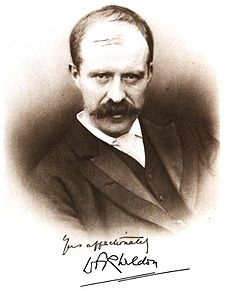
\includegraphics[width=\textwidth]{6-3_chisq_gof/figures/dice/weldon}
\end{center}
}
\begin{itemize}

\item It was observed that 5s or 6s occurred more often than expected, and Pearson hypothesized that this was probably due to the construction of the dice. Most inexpensive dice have hollowed-out pips, and since opposite sides add to 7, the face with 6 pips is lighter than its opposing face, which has only 1 pip.

\end{itemize}

\end{frame}

%%%%%%%%%%%%%%%%%%%%%%%%%%%%%%%%%%%

\begin{frame}
\frametitle{Labby's dice}

\twocol{0.5}{0.5}
{
\begin{itemize}

\item In 2009, Zacariah Labby (U of Chicago), repeated Weldon's experiment using a homemade dice-throwing, pip counting machine.
\begin{center}
\webURL{http://www.youtube.com/watch?v=95EErdouO2w}
\end{center}

\item The rolling-imaging process took about 20 seconds per roll.

\end{itemize}
}
{
\begin{center}
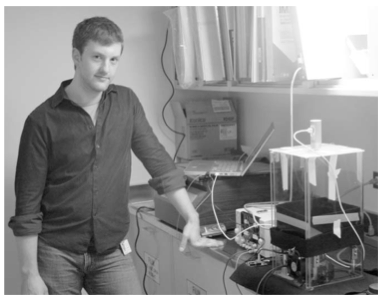
\includegraphics[width=\textwidth]{6-3_chisq_gof/figures/dice/labby}
\end{center}
}

\begin{itemize}

\item Each day there were $\sim$150 images to process manually.

\item At this rate Weldon's experiment was repeated in a little more than six full days.

\item Recommended reading: \webURL{http://galton.uchicago.edu/about/docs/labby09dice.pdf}

\end{itemize}

\end{frame}

%%%%%%%%%%%%%%%%%%%%%%%%%%%%%%%%%%%

\begin{frame}
\frametitle{Labby's dice (cont.)}

\begin{itemize}

\item Labby did not actually observe the same phenomenon that Weldon observed (higher frequency of 5s and 6s).

\item Automation allowed Labby to collect more data than Weldon did in 1894, instead of recording ``successes" and ``failures", Labby recorded the individual number of pips on each die.

\end{itemize}

\begin{center}
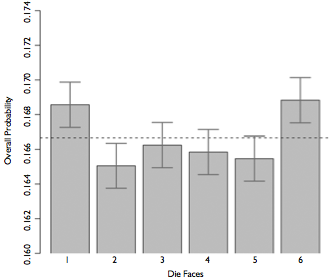
\includegraphics[width=0.55\textwidth]{6-3_chisq_gof/figures/dice/labbyPipCounts}
\end{center}

\end{frame}

%%%%%%%%%%%%%%%%%%%%%%%%%%%%%%%%%%%

\subsection*{Creating a test statistic for one-way tables}

%%%%%%%%%%%%%%%%%%%%%%%%%%%%%%%%%%%

\begin{frame}
\frametitle{Expected counts}

\pq{Labby rolled 12 dice 26,306 times. If each side is equally likely to come up, how many 1s, 2s, $\cdots$, 6s would he expect to have observed?}

\begin{enumerate}[(a)]
\item $\frac{1}{6}$
\item $\frac{12}{6}$
\item $\frac{26,306}{6}$
\solnMult{ $\frac{12 \times 26,306}{6}$ } \soln{\only<2>{\orange{$= 52,612$}}}
\end{enumerate}

\end{frame}

%%%%%%%%%%%%%%%%%%%%%%%%%%%%%%%%%%%

\begin{frame}
\frametitle{Summarizing Labby's results}

The table below shows the observed and expected counts from Labby's experiment.

{\small
\begin{center}
\renewcommand\arraystretch{1.25}
\begin{tabular}{c | c c}
Outcome	& Observed	& Expected \\
\hline
1		& 53,222		& 52,612 \\
2		& 52,118		& 52,612 \\
3		& 52,465		& 52,612 \\
4		& 52,338		& 52,612 \\
5		& 52,244		& 52,612 \\
6		& 53,285		& 52,612 \\
\hline
Total		& 315,672		& 315,672
\end{tabular}
\end{center}
}

\pause
\dq{Why are the expected counts the same for all outcomes but the observed counts are different? At a first glance, does there appear to be an inconsistency between the observed and expected counts?}

\end{frame}

%%%%%%%%%%%%%%%%%%%%%%%%%%%%%%%%%%%

\begin{frame}
\frametitle{Setting the hypotheses}

\dq{Do these data provide convincing evidence of an inconsistency between the observed and expected counts?}

\pause

\begin{itemize}
\item[$H_0$:] There is no inconsistency between the observed and the expected counts. \hlGr{The observed counts follow the same distribution as the expected counts.}

\pause

\item[$H_A$:] There is an inconsistency between the observed and the expected counts. \hlGr{The observed counts \orange{do not} follow the same distribution as the expected counts.} There is a bias in which side comes up on the roll of a die.
\end{itemize}

\end{frame}

%%%%%%%%%%%%%%%%%%%%%%%%%%%%%%%%%%%

\begin{frame}
\frametitle{Evaluating the hypotheses}

\begin{itemize}

\item To evaluate these hypotheses, we quantify how different the observed counts are from the expected counts. 

\pause

\item Large deviations from what would be expected based on sampling variation (chance) alone provide strong evidence for the alternative hypothesis.

\pause

\item This is called a \hl{goodness of fit} test since we're evaluating how well the observed data fit the expected distribution.

\end{itemize}

\end{frame}

%%%%%%%%%%%%%%%%%%%%%%%%%%%%%%%%%%%

\subsection{The chi-square test statistic}

%%%%%%%%%%%%%%%%%%%%%%%%%%%%%%%%%%%

\begin{frame}
\frametitle{Anatomy of a test statistic}

\begin{itemize}

\item The general form of a test statistic is
\[ \frac{\text{point estimate} - \text{null value}}{\text{SE of point estimate}} \]

\pause

\item This construction is based on 
\begin{enumerate}
\item identifying the difference between a point estimate and an expected value if the null hypothesis was true, and 
\item standardizing that difference using the standard error of the point estimate. 
\end{enumerate}
\pause

These two ideas will help in the construction of an appropriate test statistic for count data.

\end{itemize}

\end{frame}

%%%%%%%%%%%%%%%%%%%%%%%%%%%%%%%%%%%

\begin{frame}
\frametitle{Chi-square statistic}

When dealing with counts and investigating how far the observed counts are from the expected counts, we use a new test statistic called the \hl{chi-square ($\chi^2$) statistic}.

$\:$ \\

\pause

\formula{$\chi^2$ statistic}
{
\[\chi^2 = \sum_{i = 1}^k \frac{(O - E)^2}{E} \qquad \text{where $k$ = total number of cells} \]
}

\end{frame}

%%%%%%%%%%%%%%%%%%%%%%%%%%%%%%%%%%%

\begin{frame}
\frametitle{Calculating the chi-square statistic}

\begin{center}
\renewcommand\arraystretch{1.8}
\begin{tabular}{c | c c | c}
Outcome	& Observed	& Expected 	& $\frac{(O - E)^2}{E}$\\
\hline
1		& 53,222		& 52,612 		& $\frac{(53,222 - 52,612)^2}{52,612} = 7.07$ \\
\pause
2		& 52,118		& 52,612 		& $\frac{(52,118 - 52,612)^2}{52,612} = 4.64$ \\
\pause
3		& 52,465		& 52,612 		& $\frac{(52,465 - 52,612)^2}{52,612} = 0.41$ \\
\pause
4		& 52,338		& 52,612 		& $\frac{(52,338 - 52,612)^2}{52,612} = 1.43$\\
\pause
5		& 52,244		& 52,612 		& $\frac{(52,244 - 52,612)^2}{52,612} = 2.57$\\
\pause
6		& 53,285		& 52,612 		& $\frac{(53,285 - 52,612)^2}{52,612} = 8.61$\ \\
\hline
\pause
Total		& 315,672		& 315,672		& 24.73
\end{tabular}
\end{center}

\end{frame}

%%%%%%%%%%%%%%%%%%%%%%%%%%%%%%%%%%%

\begin{frame}
\frametitle{Why square?}


Squaring the difference between the observed and the expected outcome does two things:
\pause
\begin{itemize}
\item Any standardized difference that is squared will now be positive.
\pause
\item Differences that already looked unusual will become much larger after being squared.
\end{itemize}

\vspace{1cm}

\pause
\dq{When have we seen this before?}

\end{frame}

%%%%%%%%%%%%%%%%%%%%%%%%%%%%%%%%%%%

\subsection{The chi-square distribution and finding areas}

%%%%%%%%%%%%%%%%%%%%%%%%%%%%%%%%%%%

\begin{frame}
\frametitle{The chi-square distribution}

\begin{itemize}

\item In order to determine if the $\chi^2$ statistic we calculated is considered unusually high or not we need to first describe its distribution.

\pause

\item The chi-square distribution has just one parameter called \hl{degrees of freedom (df)}, which influences the shape, center, and spread of the distribution. \\

\end{itemize}

\pause

$\:$ \\

\Remember{So far we've seen three other continuous distributions:
\begin{itemize}
\item[-] normal distribution: unimodal and symmetric with two parameters: mean and standard deviation
\item[-] T distribution: unimodal and symmetric with one parameter: degrees of freedom
\item[-] F distribution: unimodal and right skewed with two parameters: degrees of freedom or numerator (between group variance) and denominator (within group variance)
\end{itemize}
}

\end{frame}

%%%%%%%%%%%%%%%%%%%%%%%%%%%%%%%%%%%

\begin{frame}
\frametitle{}

\pq{Which of the following is false?}

\begin{center}
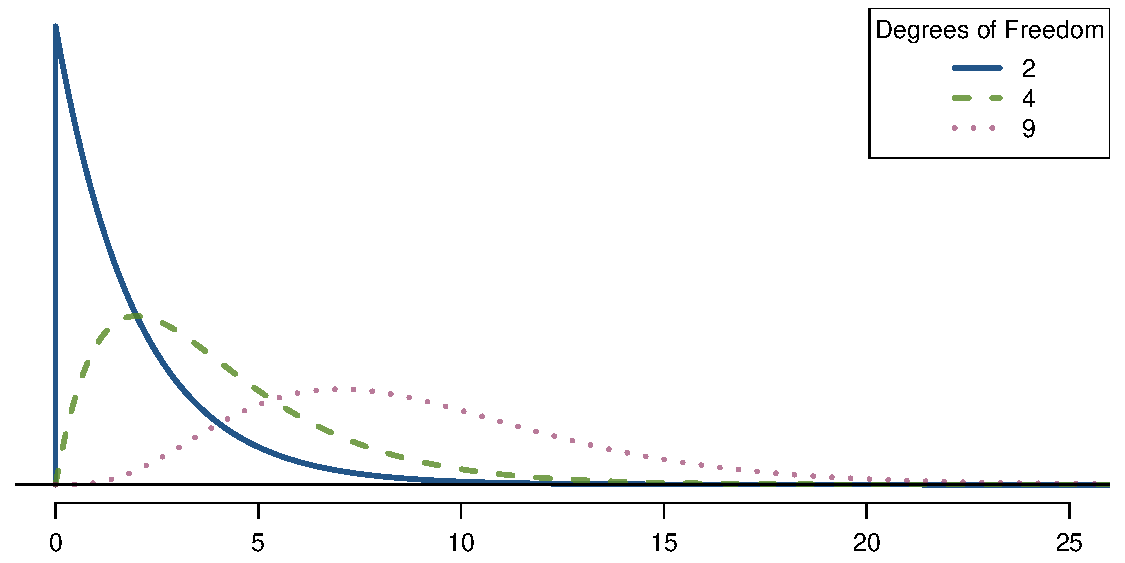
\includegraphics[width=0.7\textwidth]{6-3_chisq_gof/figures/chiSquareDistributionWithInceasingDF/chiSquareDistributionWithInceasingDF}
\end{center}

As the df increases,
\begin{enumerate}[(a)]
\item the center of the $\chi^2$ distribution increases as well
\item the variability of the $\chi^2$ distribution increases as well
\solnMult{the shape of the $\chi^2$ distribution becomes more skewed (less like a normal)}
\end{enumerate}

\end{frame}

%%%%%%%%%%%%%%%%%%%%%%%%%%%%%%%%%%%

\begin{frame}[fragile]
\frametitle{Finding areas under the chi-square curve}

\begin{itemize}

\item p-value = tail area under the chi-square distribution (as usual)

\pause

\item For this we can use technology, or a \hl{chi-square probability table}.

\pause

\item  This table works a lot like the $t$ table, but only provides upper tail values.
\end{itemize}

\begin{center}
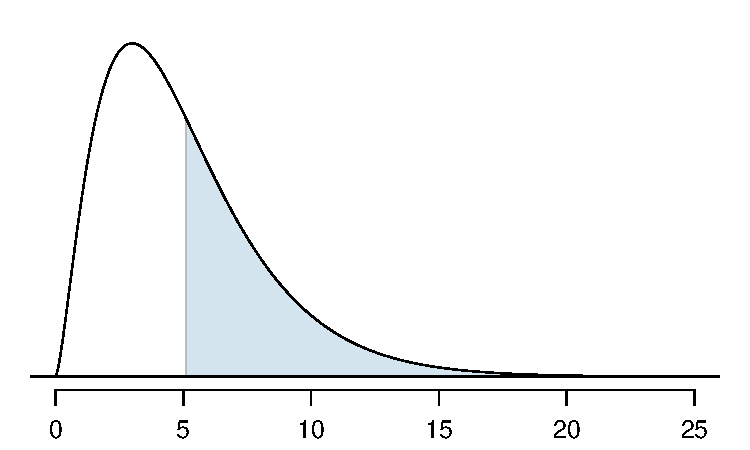
\includegraphics[width=0.3\textwidth]{6-3_chisq_gof/figures/above5Point1WithDF5/above5Point1WithDF5}
\end{center}

{\scriptsize
\begin{center}
\begin{tabular}{r | rrrr | rrrr |}
  \hline
Upper tail & 0.3 & 0.2 & 0.1 & 0.05 & 0.02 & 0.01 & 0.005 & 0.001 \\ 
  \hline
df \hfill 1 &  1.07 &  1.64 &  2.71 &  3.84 &  5.41 &  6.63 &  7.88 &  10.83 \\ 
  2 &  2.41 &  3.22 &  4.61 &  5.99 &  7.82 &  9.21 &  10.60 &  13.82 \\ 
  3 &  3.66 &  4.64 &  6.25 &  7.81 &  9.84 &  11.34 &  12.84 &  16.27 \\ 
  4 &  4.88 &  5.99 &  7.78 &  9.49 &  11.67 &  13.28 &  14.86 &  18.47 \\ 
  5 &  6.06 &  7.29 &  9.24 &  11.07 &  13.39 &  15.09 &  16.75 &  20.52 \\ 
  \hline
  6 &  7.23 &  8.56 &  10.64 &  12.59 &  15.03 &  16.81 &  18.55 &  22.46 \\ 
  7 &  8.38 &  9.80 &  12.02 &  14.07 &  16.62 &  18.48 &  20.28 &  24.32 \\ 
  $\cdots$ &   &   &   &   &   &   &   &   \\ 
\end{tabular}
\end{center}
}

\end{frame}

%%%%%%%%%%%%%%%%%%%%%%%%%%%%%%%%%%%

\begin{frame}
\frametitle{Finding areas under the chi-square curve (cont.)}

\dq{Estimate the shaded area under the chi-square curve with $df = 6$.}

\twocol{0.6}{0.4}{
\begin{center}
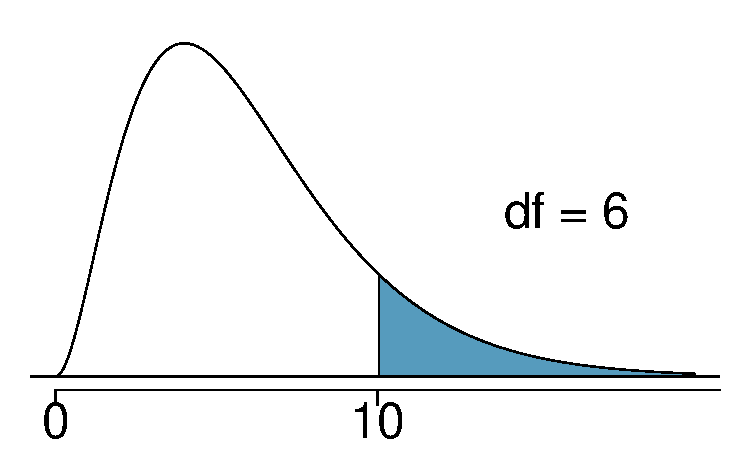
\includegraphics[width=0.67\textwidth]{6-3_chisq_gof/figures/above10WithDF6/above10WithDF6}
\end{center}
}
{\only<4 |handout:0>{\orange{$P(\chi^2_{df = 6} > 10)$\\ is between 0.1 and 0.2}}
}

\only<1>{
\begin{center}
{\footnotesize
\begin{tabular}{r | rrrr | rrrr |}
  \hline
Upper tail & 0.3 & 0.2 & 0.1 & 0.05 & 0.02 & 0.01 & 0.005 & 0.001 \\ 
  \hline
df \hfill 1 &  1.07 &  1.64 &  2.71 &  3.84 &  5.41 &  6.63 &  7.88 &  10.83 \\ 
  2 &  2.41 &  3.22 &  4.61 &  5.99 &  7.82 &  9.21 &  10.60 &  13.82 \\ 
  3 &  3.66 &  4.64 &  6.25 &  7.81 &  9.84 &  11.34 &  12.84 &  16.27 \\ 
  4 &  4.88 &  5.99 &  7.78 &  9.49 &  11.67 &  13.28 &  14.86 &  18.47 \\ 
  5 &  6.06 &  7.29 &  9.24 &  11.07 &  13.39 &  15.09 &  16.75 &  20.52 \\ 
  \hline
  6 &  7.23 &  8.56 &   10.64  &  12.59 &  15.03 &  16.81 &  18.55 &  22.46 \\ 
  7 &  8.38 &  9.80 &  12.02 &  14.07 &  16.62 &  18.48 &  20.28 &  24.32 \\ 
  \hline
\end{tabular}
}
\end{center}
}

\only<2 | handout:0>{
\begin{center}
{\footnotesize
\begin{tabular}{r | rrrr | rrrr |}
  \hline
Upper tail & 0.3 & 0.2 & 0.1 & 0.05 & 0.02 & 0.01 & 0.005 & 0.001 \\ 
  \hline
df \hfill 1 &  1.07 &  1.64 &  2.71 &  3.84 &  5.41 &  6.63 &  7.88 &  10.83 \\ 
  2 &  2.41 &  3.22 &  4.61 &  5.99 &  7.82 &  9.21 &  10.60 &  13.82 \\ 
  3 &  3.66 &  4.64 &  6.25 &  7.81 &  9.84 &  11.34 &  12.84 &  16.27 \\ 
  4 &  4.88 &  5.99 &  7.78 &  9.49 &  11.67 &  13.28 &  14.86 &  18.47 \\ 
  5 &  6.06 &  7.29 &  9.24 &  11.07 &  13.39 &  15.09 &  16.75 &  20.52 \\ 
  \hline
\rowcolor[gray]{.6}
  6 &  7.23 &  8.56 &   10.64  &  12.59 &  15.03 &  16.81 &  18.55 &  22.46 \\ 
  7 &  8.38 &  9.80 &  12.02 &  14.07 &  16.62 &  18.48 &  20.28 &  24.32 \\ 
  \hline
\end{tabular}
}
\end{center}
}

\only<3 | handout:0>{
\begin{center}
{\footnotesize
\begin{tabular}{r | rrrr | rrrr |}
  \hline
Upper tail & 0.3 & 0.2 & 0.1 & 0.05 & 0.02 & 0.01 & 0.005 & 0.001 \\ 
  \hline
df \hfill 1 &  1.07 &  1.64 &  2.71 &  3.84 &  5.41 &  6.63 &  7.88 &  10.83 \\ 
  2 &  2.41 &  3.22 &  4.61 &  5.99 &  7.82 &  9.21 &  10.60 &  13.82 \\ 
  3 &  3.66 &  4.64 &  6.25 &  7.81 &  9.84 &  11.34 &  12.84 &  16.27 \\ 
  4 &  4.88 &  5.99 &  7.78 &  9.49 &  11.67 &  13.28 &  14.86 &  18.47 \\ 
  5 &  6.06 &  7.29 &  9.24 &  11.07 &  13.39 &  15.09 &  16.75 &  20.52 \\ 
  \hline
  \rowcolor[gray]{.6}
  6 &  7.23 & \orange{ 8.56 }&  \orange{ 10.64 } &  12.59 &  15.03 &  16.81 &  18.55 &  22.46 \\ 
  7 &  8.38 &  9.80 &  12.02 &  14.07 &  16.62 &  18.48 &  20.28 &  24.32 \\ 
  \hline
\end{tabular}
}
\end{center}
}

\only<4 | handout:0>{
\begin{center}
{\footnotesize
\begin{tabular}{r | r >{\columncolor[gray]{0.6}[.5\tabcolsep]}r >{\columncolor[gray]{0.6}[.5\tabcolsep]}rr | rrrr |}
  \hline
Upper tail & 0.3 & \orange{0.2} & \orange{0.1} & 0.05 & 0.02 & 0.01 & 0.005 & 0.001 \\ 
  \hline
df \hfill 1 &  1.07 &  1.64 &  2.71 &  3.84 &  5.41 &  6.63 &  7.88 &  10.83 \\ 
  2 &  2.41 &  3.22 &  4.61 &  5.99 &  7.82 &  9.21 &  10.60 &  13.82 \\ 
  3 &  3.66 &  4.64 &  6.25 &  7.81 &  9.84 &  11.34 &  12.84 &  16.27 \\ 
  4 &  4.88 &  5.99 &  7.78 &  9.49 &  11.67 &  13.28 &  14.86 &  18.47 \\ 
  5 &  6.06 &  7.29 &  9.24 &  11.07 &  13.39 &  15.09 &  16.75 &  20.52 \\ 
  \hline
  \rowcolor[gray]{.6}
  6 &  7.23 & \orange{ 8.56 }&  \orange{ 10.64 } &  12.59 &  15.03 &  16.81 &  18.55 &  22.46 \\ 
  7 &  8.38 &  9.80 &  12.02 &  14.07 &  16.62 &  18.48 &  20.28 &  24.32 \\ 
  \hline
\end{tabular}
}
\end{center}
}

\end{frame}

%%%%%%%%%%%%%%%%%%%%%%%%%%%%%%%%%%%

\begin{frame}
\frametitle{Finding areas under the chi-square curve (cont.)}

\pq{Estimate the shaded area (above 17) under the $\chi^2$ curve with $df = 9$.}

\twocol{0.6}{0.4}{
\begin{center}
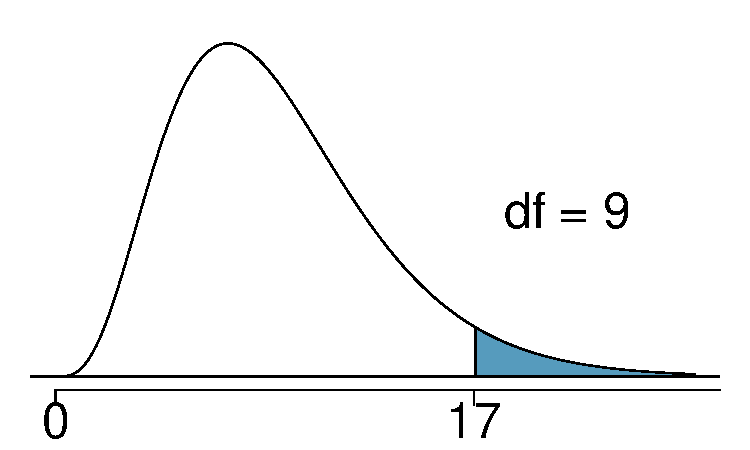
\includegraphics[width=0.67\textwidth]{6-3_chisq_gof/figures/above17WithDF9/above17WithDF9}
\end{center}
}
{
{\small
\begin{enumerate}[(a)]
\setlength{\itemsep}{0in}
\item 0.05
\item 0.02
\solnMult{between 0.02 and 0.05}
\item between 0.05 and 0.1
\item between 0.01 and 0.02
\end{enumerate}
}
}

\only<1>{
\begin{center}
{\scriptsize
\begin{tabular}{r | rrrr | rrrr |}
  \hline
Upper tail & 0.3 & 0.2 & 0.1 & 0.05 & 0.02 & 0.01 & 0.005 & 0.001 \\ 
  \hline
df  \hfill 7 &  8.38 &  9.80 &  12.02 &  14.07 &  16.62 &  18.48 &  20.28 &  24.32 \\ 
  8 &  9.52 &  11.03 &  13.36 &  15.51 &  18.17 &  20.09 &  21.95 &  26.12 \\ 
  9 &  10.66 &  12.24 &  14.68 &  16.92 &  19.68 &  21.67 &  23.59 &  27.88 \\ 
  10 &  11.78 &  13.44 &  15.99 &  18.31 &  21.16 &  23.21 &  25.19 &  29.59 \\ 
  \hline
  11 &   12.90 &  14.63 &  17.28 &  19.68 &  22.62 &  24.72 &  26.76 &  31.26 \\ 
\end{tabular}
}
\end{center}
}

\only<2 | handout:0>{
\begin{center}
{\scriptsize
\begin{tabular}{r | rrr >{\columncolor[gray]{0.6}[.5\tabcolsep]}r | >{\columncolor[gray]{0.6}[.5\tabcolsep]}rrrr |}
  \hline
Upper tail & 0.3 & 0.2 & 0.1 & \orange{ 0.05 } & \orange{ 0.02 } & 0.01 & 0.005 & 0.001 \\ 
  \hline
df  \hfill 7 &  8.38 &  9.80 &  12.02 &  14.07 &  16.62 &  18.48 &  20.28 &  24.32 \\ 
  8 &  9.52 &  11.03 &  13.36 &  15.51 &  18.17 &  20.09 &  21.95 &  26.12 \\ 
    \rowcolor[gray]{.6}
  9 &  10.66 &  12.24 &  14.68 &  \orange{16.92 }&  \orange{19.68} &  21.67 &  23.59 &  27.88 \\ 
  10 &  11.78 &  13.44 &  15.99 &  18.31 &  21.16 &  23.21 &  25.19 &  29.59 \\ 
  \hline
  11 &   12.90 &  14.63 &  17.28 &  19.68 &  22.62 &  24.72 &  26.76 &  31.26 \\ 
  \hline
\end{tabular}
}
\end{center}
}

\end{frame}

%%%%%%%%%%%%%%%%%%%%%%%%%%%%%%%%%%%

\begin{frame}
\frametitle{Finding areas under the chi-square curve (one more)}

\pq{Estimate the shaded area (above 30) under the $\chi^2$ curve with $df = 10$.}

\twocol{0.6}{0.4}{
\begin{center}
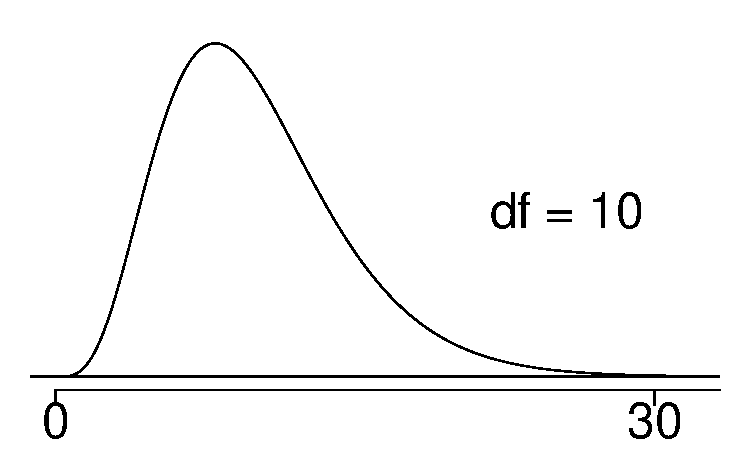
\includegraphics[width=0.67\textwidth]{6-3_chisq_gof/figures/above30WithDF10/above30WithDF10}
\end{center}
}
{
{\small
\begin{enumerate}[(a)]
\setlength{\itemsep}{0in}
\item greater than 0.3
\item between 0.005 and 0.001
\solnMult{less than 0.001}
\item greater than 0.001
\item cannot tell using this table
\end{enumerate}
}
}

\only<1>{
\begin{center}
{\scriptsize
\begin{tabular}{r | rrrr | rrrr |}
  \hline
Upper tail & 0.3 & 0.2 & 0.1 & 0.05 & 0.02 & 0.01 & 0.005 & 0.001 \\ 
  \hline
df  \hfill 7 &  8.38 &  9.80 &  12.02 &  14.07 &  16.62 &  18.48 &  20.28 &  24.32 \\ 
  8 &  9.52 &  11.03 &  13.36 &  15.51 &  18.17 &  20.09 &  21.95 &  26.12 \\ 
  9 &  10.66 &  12.24 &  14.68 &  16.92 &  19.68 &  21.67 &  23.59 &  27.88 \\ 
  10 &  11.78 &  13.44 &  15.99 &  18.31 &  21.16 &  23.21 &  25.19 &  29.59 \\ 
  \hline
  11 &   12.90 &  14.63 &  17.28 &  19.68 &  22.62 &  24.72 &  26.76 &  31.26 \\ 
\end{tabular}
}
\end{center}
}

\only<2 | handout:0>{
\begin{center}
{\scriptsize
\begin{tabular}{r | rrrr | rrr>{\columncolor[gray]{0.6}[.5\tabcolsep]}r | c}
  \cline{1-9}
Upper tail & 0.3 & 0.2 & 0.1 & 0.05 &  0.02  & 0.01 & 0.005 & \orange{0.001} & \mathhl{\rightarrow}  \\ 
  \cline{1-9}
df  \hfill 7 &  8.38 &  9.80 &  12.02 &  14.07 &  16.62 &  18.48 &  20.28 &  24.32 \\ 
  8 &  9.52 &  11.03 &  13.36 &  15.51 &  18.17 &  20.09 &  21.95 &  26.12 \\ 
  9 &  10.66 &  12.24 &  14.68 &  16.92 &  19.68 &  21.67 &  23.59 &  27.88 \\ 
    \rowcolor[gray]{.6}
  10 &  11.78 &  13.44 &  15.99 &  18.31 &  21.16 &  23.21 &  25.19 &  \orange{29.59} & \mathhl{\rightarrow} \\ 
  \cline{1-9}
  11 &   12.90 &  14.63 &  17.28 &  19.68 &  22.62 &  24.72 &  26.76 &  31.26 \\ 
  \cline{1-9}
\end{tabular}
}
\end{center}
}

\end{frame}

%%%%%%%%%%%%%%%%%%%%%%%%%%%%%%%%%%%

\begin{frame}[fragile]
\frametitle{Finding the tail areas using computation}

\begin{itemize}

\item While probability tables are very helpful in understanding how probability distributions work, and provide quick reference when computational resources are not available, they are somewhat archaic.

\pause

\item Using R:
{\footnotesize
\begin{lstlisting}
pchisq(q = 30, df = 10, lower.tail = FALSE)
# 0.0008566412
\end{lstlisting}
}

\pause

\item Using a web applet:

\webURL{http://bitly.com/dist_calc}

\end{itemize}

\end{frame}

%%%%%%%%%%%%%%%%%%%%%%%%%%%%%%%%%%%

\subsection{Finding a p-value for a chi-square test}

%%%%%%%%%%%%%%%%%%%%%%%%%%%%%%%%%%%

\begin{frame}
\frametitle{Back to Labby's dice}

\begin{itemize}

\item The research question was: Do these data provide convincing evidence of an inconsistency between the observed and expected counts?

\pause

\item The hypotheses were:
\begin{itemize}
\item[$H_0$:] There is no inconsistency between the observed and the expected counts. The observed counts follow the same distribution as the expected counts.
\item[$H_A$:] There is an inconsistency between the observed and the expected counts. The observed counts \orange{do not} follow the same distribution as the expected counts. There is a bias in which side comes up on the roll of a die.
\end{itemize}

\pause

\item We had calculated a test statistic of \orange{$\chi^2 = 24.67$}.

\pause

\item All we need is the $df$ and we can calculate the tail area (the p-value) and make a decision on the hypotheses.

\end{itemize}

\end{frame}

%%%%%%%%%%%%%%%%%%%%%%%%%%%%%%%%%%%

\begin{frame}
\frametitle{Degrees of freedom for a goodness of fit test}

\begin{itemize}

\item When conducting a goodness of fit test to evaluate how well the observed data follow an expected distribution, the degrees of freedom are calculated as the number of cells ($k$) minus 1.
\[ \mathhl{df = k - 1} \]

\pause

\item For dice outcomes, $k = 6$, therefore
\[ df = 6 - 1 = 5 \]

\end{itemize}

\end{frame}

%%%%%%%%%%%%%%%%%%%%%%%%%%%%%%%%%%%

\begin{frame}
\frametitle{Finding a p-value for a chi-square test}

The \hl{p-value} for a chi-square test is defined as the \hl{tail area above the calculated test statistic}.

\twocol{0.6}{0.4}{
\begin{center}
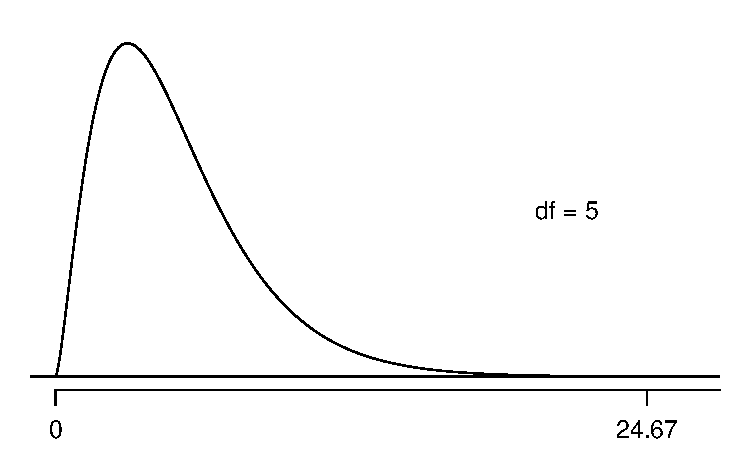
\includegraphics[width=0.67\textwidth]{6-3_chisq_gof/figures/above24Point67WithDF5/above24Point67WithDF5}
\end{center}
}
{
p-value = $P(\chi^2_{df = 5} > 24.67)$\\ is less than 0.001
}

\begin{center}
{\footnotesize
\begin{tabular}{r | rrrr | rrrr r}
  \hline
Upper tail & 0.3 & 0.2 & 0.1 & 0.05 & 0.02 & 0.01 & 0.005 & 0.001 & \orange{$\rightarrow$}  \\ 
  \hline
df \hfill 1 &  1.07 &  1.64 &  2.71 &  3.84 &  5.41 &  6.63 &  7.88 &  10.83 \\ 
  2 &  2.41 &  3.22 &  4.61 &  5.99 &  7.82 &  9.21 &  10.60 &  13.82 \\ 
  3 &  3.66 &  4.64 &  6.25 &  7.81 &  9.84 &  11.34 &  12.84 &  16.27 \\ 
  4 &  4.88 &  5.99 &  7.78 &  9.49 &  11.67 &  13.28 &  14.86 &  18.47 \\ 
  \rowcolor[gray]{.6}
  5 &  6.06 &  7.29 &  9.24 &  11.07 &  13.39 &  15.09 &  16.75 &  20.52 &\orange{$\rightarrow$} \\ 
  \hline
\end{tabular}
}
\end{center}

\end{frame}

%%%%%%%%%%%%%%%%%%%%%%%%%%%%%%%%%%%

\begin{frame}
\frametitle{Conclusion of the hypothesis test}

\pq{We calculated a p-value less than 0.001. At 5\% significance level, what is the conclusion of the hypothesis test?}

\begin{enumerate}[(a)]
\item Reject $H_0$, the data provide convincing evidence that the dice are fair.
\solnMult{Reject $H_0$, the data provide convincing evidence that the dice are biased.}
\item Fail to reject $H_0$, the data provide convincing evidence that the dice are fair.
\item Fail to reject $H_0$, the data provide convincing evidence that the dice are biased.
\end{enumerate}

\end{frame}

%%%%%%%%%%%%%%%%%%%%%%%%%%%%%%%%%%%

\begin{frame}
\frametitle{Turns out...}

\begin{itemize}

\item The 1-6 axis is consistently shorter than the other two (2-5 and 3-4), thereby supporting the hypothesis that the faces with one and six pips are larger than the other faces.

\item Pearson's claim that 5s and 6s appear more often due to the carved-out pips is not supported by these data.

\item Dice used in casinos have flush faces, where the pips are filled in with a plastic of the same density as the surrounding material and are precisely balanced.

\end{itemize}

\begin{center}
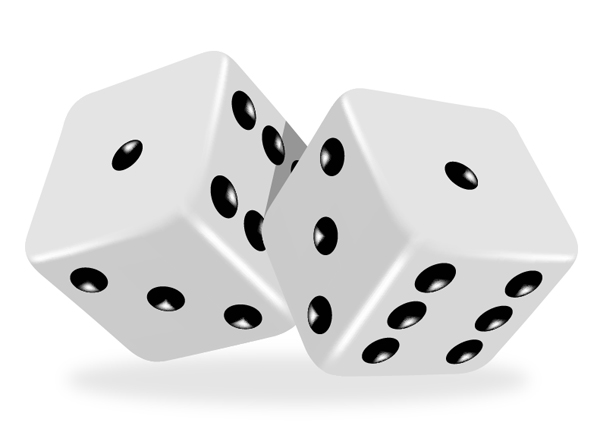
\includegraphics[width=0.3\textwidth]{6-3_chisq_gof/figures/dice/regular}
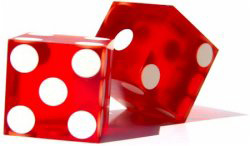
\includegraphics[width=0.3\textwidth]{6-3_chisq_gof/figures/dice/casino}
\end{center}


\end{frame}

%%%%%%%%%%%%%%%%%%%%%%%%%%%%%%%%%%%

\begin{frame}
\frametitle{Recap: p-value for a chi-square test}

\begin{itemize}

\item The p-value for a chi-square test is defined as the tail area \hl{above} the calculated test statistic.

\item This is because the test statistic is always positive, and a higher test statistic means a stronger deviation from the null hypothesis.

\end{itemize}

\begin{center}
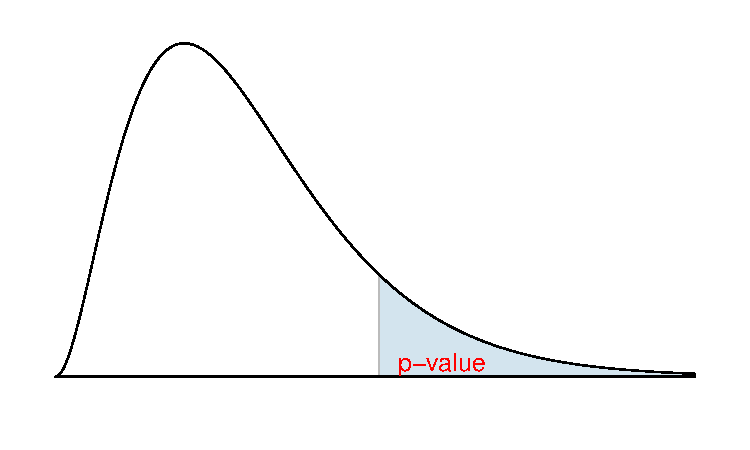
\includegraphics[width=0.7\textwidth]{6-3_chisq_gof/figures/genericChiSquare/genericChiSquare}
\end{center}

\end{frame}

%%%%%%%%%%%%%%%%%%%%%%%%%%%%%%%%%%%

\begin{frame}
\frametitle{Conditions for the chi-square test}

\begin{enumerate}

\item \hlGr{Independence:} Each case that contributes a count to the table must be independent of all the other cases in the table.

\pause

\item \hlGr{Sample size:} Each particular scenario (i.e. cell) must have at least 5 \orange{expected} cases.

\pause

\item \hlGr{df $>$ 1:} Degrees of freedom must be greater than 1.

\end{enumerate}

\pause

Failing to check conditions may unintentionally affect the test's error rates.

\end{frame}

%%%%%%%%%%%%%%%%%%%%%%%%%%%%%%%%%%%

\subsection{2009 Iran Election}

%%%%%%%%%%%%%%%%%%%%%%%%%%%%%%%%%%%

\begin{frame}
\frametitle{2009 Iran Election}

\dq{There was lots of talk of election fraud in the 2009 Iran election. We'll compare the data from a poll conducted before the election (observed data) to the reported votes in the election to see if the two follow the same distribution.}

\begin{center}
\begin{tabular}{l | r r}
					& \footnotesize{Observed \# of} & \footnotesize{Reported \% of} \\
\footnotesize{Candidate}	& \footnotesize{voters in poll} & \footnotesize{votes in election} \\
\hline
(1) Ahmedinajad	& 338	& 63.29\% \\
(2) Mousavi		& 136	& 34.10\% \\
(3) Minor candidates	& 30	& 2.61\% \\
\hline
Total			& 504	& 100\% \\
\pause
			& \hl{$\downarrow$}	& \hl{$\downarrow$}	\\
			& \hl{observed}	& \hl{expected} \\
			& 			& \hl{distribution} 	
\end{tabular}
\end{center}

\end{frame}

%%%%%%%%%%%%%%%%%%%%%%%%%%%%%%%%%%%

\begin{frame}
\frametitle{Hypotheses}

\dq{What are the hypotheses for testing if the distributions of reported and polled votes are different?}

\soln{
\only<2>{
\begin{itemize}
\item[$H_0$:] The observed counts from the poll follow the same distribution as the reported votes.
\item[$H_A$:] The observed counts from the poll do not follow the same distribution as the reported votes.
\end{itemize}
}}

\end{frame}

%%%%%%%%%%%%%%%%%%%%%%%%%%%%%%%%%%%

\begin{frame}
\frametitle{Calculation of the test statistic}

{\small
\begin{center}
\begin{tabular}{l | r r r}
					& \footnotesize{Observed \# of} & \footnotesize{Reported \% of}	& \footnotesize{Expected \# of} \\
\footnotesize{Candidate}	& \footnotesize{voters in poll} & \footnotesize{votes in election}		&  \footnotesize{votes in poll} \\
\hline
\footnotesize{(1) Ahmedinajad}	& 338	& 63.29\% 	& 504 $\times$ 0.6329 = 319 \\
\footnotesize{(2) Mousavi}		& 136	& 34.10\%		& 504 $\times$ 0.3410 = 172 \\
\footnotesize{(3) Minor candidates}	& 30	& 2.61\% 		& 504 $\times$ 0.0261 = 13\\
\hline
Total			& 504	& 100\%		& 504
\end{tabular}
\end{center}
}

\pause

\begin{eqnarray*}
\frac{(O_1 - E_1)^2}{E_1} = \frac{(338 - 319)^2}{319} &=& 1.13 \\
\pause
\frac{(O_2 - E_2)^2}{E_2} = \frac{(136 - 172)^2}{172} &=& 7.53 \\
\pause
\frac{(O_2 - E_2)^2}{E_2} = \frac{(30 - 13)^2}{13} &=& 22.23 \\
\pause
 \chi^2_{\mathhl{df = 3 - 1 = 2}} &=& 30.89
\end{eqnarray*}


\end{frame}

%%%%%%%%%%%%%%%%%%%%%%%%%%%%%%%%%%%

\begin{frame}
\frametitle{Conclusion}

\pq{Based on these calculations what is the conclusion of the hypothesis test?}

\begin{enumerate}[(a)]
\solnMult{p-value is low, $H_0$ is rejected. The observed counts from the poll do \underline{not} follow the same distribution as the reported votes.}
\item p-value is high, $H_0$ is not rejected. The observed counts from the poll follow the same distribution as the reported votes.
\item p-value is low, $H_0$ is rejected. The observed counts from the poll follow the same distribution as the reported votes
\item p-value is low, $H_0$ is not rejected. The observed counts from the poll do \underline{not} follow the same distribution as the reported votes.
\end{enumerate}

\end{frame}
